% ============================================================================
% CHAPTER 5: MULTI-LAYER PERCEPTRONS
% ============================================================================

\chapter{Multi-Layer Perceptrons}
\label{ch:mlp}

% ============================================================================
% OVERVIEW
% ============================================================================

\section{Chapter Overview}

This chapter introduces \textbf{Multi-Layer Perceptrons (MLPs)}---neural networks with multiple layers that can solve non-linearly separable problems. We establish formal definitions of network depth, layers, and notation that will be used throughout our study of deep learning.

\textbf{Learning Objectives:}
\begin{itemize}
    \item Understand why multiple layers are needed
    \item Define depth and layers using graph theory
    \item Master standard neural network notation
    \item Trace information flow through deep networks
    \item Understand the matrix formulation of neural networks
\end{itemize}

% ============================================================================
% PERCEPTRON CONVERGENCE PROOF
% ============================================================================

\section{Perceptron Convergence Proof}

In the previous chapter, we introduced the Perceptron learning algorithm and stated the premise for its convergence. Now, we provide the formal mathematical proof that the algorithm will find a separating hyperplane in a finite number of steps if the data is linearly separable.

\subsection{Setup and Normalization}

Let $\mathcal{P}, \mathcal{N} \subset \R^n$ be our finite sets of positive and negative points. For mathematical convenience, we can convert every negative point $\vect{x} \in \mathcal{N}$ into a positive point by taking its negation, $-\vect{x}$. Let $\mathcal{P}' = \mathcal{P} \cup \{-\vect{x} \mid \vect{x} \in \mathcal{N}\}$. 
Now, the linear separability condition simplifies to finding a weight vector $\vect{w}^*$ such that:
\[
(\vect{w}^*)^\top \vect{p} \geq 0 \quad \text{for all } \vect{p} \in \mathcal{P}'
\]
Next, we normalize all vectors $\vect{p} \in \mathcal{P}'$ such that their magnitude $\|\vect{p}\| = 1$. Let $\delta$ be the smallest dot product between the optimal weights $\vect{w}^*$ and any point $\vect{p} \in \mathcal{P}'$:
\[
\delta = \min_{\vect{p} \in \mathcal{P}'} (\vect{w}^*)^\top \vect{p}
\]
Since the data is strictly separable, $\delta > 0$.

\subsection{The Proof}

Assume we initialize the perceptron with $\vect{w}_0 = \vect{0}$. 
In each step $t$ where a mistake is made on point $\vect{p}$, we update the weights:
\[
\vect{w}_{t+1} = \vect{w}_t + \vect{p}
\]
To prove convergence, we analyze the cosine of the angle $\beta$ between our current weight vector $\vect{w}_{t+1}$ and the optimal normalizer $\vect{w}^*$:
\[
\cos \beta = \frac{(\vect{w}^*)^\top \vect{w}_{t+1}}{\|\vect{w}^*\| \|\vect{w}_{t+1}\|}
\]
By evaluating the numerator recursively:
\[
(\vect{w}^*)^\top \vect{w}_{t+1} = (\vect{w}^*)^\top (\vect{w}_t + \vect{p}) = (\vect{w}^*)^\top \vect{w}_t + (\vect{w}^*)^\top \vect{p} \geq (\vect{w}^*)^\top \vect{w}_t + \delta
\]
After $M$ updates, $(\vect{w}^*)^\top \vect{w}_M \geq M \delta$.

By evaluating the denominator squared:
\[
\|\vect{w}_{t+1}\|^2 = \|\vect{w}_t + \vect{p}\|^2 = \|\vect{w}_t\|^2 + \|\vect{p}\|^2 + 2\vect{w}_t^\top \vect{p}
\]
Since the update only happens when there is a mistake, $\vect{w}_t^\top \vect{p} \leq 0$. And because we normalized $\|\vect{p}\| = 1$, we get:
\[
\|\vect{w}_{t+1}\|^2 \leq \|\vect{w}_t\|^2 + 1
\]
After $M$ updates, $\|\vect{w}_M\|^2 \leq M$, so $\|\vect{w}_M\| \leq \sqrt{M}$.

Putting it together:
\[
\cos \beta = \frac{(\vect{w}^*)^\top \vect{w}_M}{\|\vect{w}^*\| \|\vect{w}_M\|} \geq \frac{M \delta}{\|\vect{w}^*\| \sqrt{M}} = \frac{\sqrt{M} \delta}{\|\vect{w}^*\|}
\]
Since $\cos \beta$ must be $\leq 1$, we have:
\[
\frac{\sqrt{M} \delta}{\|\vect{w}^*\|} \leq 1 \implies M \leq \frac{\|\vect{w}^*\|^2}{\delta^2}
\]
This proves that the maximum number of updates $M$ is finite and bounded. Thus, the perceptron learning algorithm will always converge!

% ============================================================================
% BINARIZING REAL-WORLD APPLICATIONS
% ============================================================================

\section{Binarizing Real-World Applications}

Before moving to more complex multi-layered architectures, let us observe how standard binary perceptrons are utilized for real-world scenarios. Many physical problems provide continuous feature variables, yet basic network models traditionally handle binary input representations flawlessly.

Consider an e-commerce platform predicting whether a customer will purchase a product:
\begin{itemize}
    \item $x_1$: Time spent on the product page.
    \item $x_2$: Number of related products viewed.
    \item $x_3$: Average purchase history.
\end{itemize}

To process this data linearly with standard Boolean combinations, we can \textbf{binarize} the inputs by introducing simple thresholds:
\begin{itemize}
    \item \textbf{Feature 1}: If time spent $> 10$ minutes, set $x_1 = 1$, else $0$.
    \item \textbf{Feature 2}: If related products viewed $> 3$, set $x_2 = 1$, else $0$.
    \item \textbf{Feature 3}: If average past purchase value $> \$50$, set $x_3 = 1$, else $0$.
\end{itemize}

By transforming continuous real-world data into boolean feature arrays $\vect{x} = [1, 0, 1]$, we can seamlessly utilize simple linear classifiers and logic gate formations. However, this manual categorization process is often rigid and loses nuance—which motivates the necessity for continuous, multi-layer, and non-linear network representations.

% ============================================================================
% WHY MULTIPLE LAYERS?
% ============================================================================

\section{The Need for Multiple Layers}

\subsection{The XOR Revisited}

Recall that a single perceptron cannot solve XOR because it's not linearly separable. However, XOR \textit{can} be expressed as a combination of simpler functions:

\[
\text{XOR}(x_1, x_2) = \text{AND}(\text{OR}(x_1, x_2), \text{NAND}(x_1, x_2))
\]

This suggests that by \textbf{combining multiple neurons}, we can solve problems that individual neurons cannot.

\begin{center}
\begin{tikzpicture}[
    input/.style={circle, draw, fill=blue!20, minimum size=0.8cm},
    neuron/.style={circle, draw, fill=yellow!30, minimum size=0.8cm},
    output/.style={circle, draw, fill=red!20, minimum size=0.8cm}
]
    % Inputs
    \node[input] (x1) at (0, 1.5) {$x_1$};
    \node[input] (x2) at (0, -1.5) {$x_2$};
    
    % Hidden layer
    \node[neuron] (or) at (3, 1) {OR};
    \node[neuron] (nand) at (3, -1) {NAND};
    
    % Output
    \node[output] (and) at (6, 0) {AND};
    
    % Connections
    \draw[-Stealth] (x1) -- (or);
    \draw[-Stealth] (x1) -- (nand);
    \draw[-Stealth] (x2) -- (or);
    \draw[-Stealth] (x2) -- (nand);
    \draw[-Stealth] (or) -- (and);
    \draw[-Stealth] (nand) -- (and);
    
    % Labels
    \node[above] at (6, 0.5) {XOR};
\end{tikzpicture}
\end{center}

\begin{bluebox}[Key Insight: Hierarchical Computation]
Just as the visual cortex processes information in layers (edges $\rightarrow$ shapes $\rightarrow$ objects $\rightarrow$ scenes), neural networks can build complex representations by composing simpler ones layer by layer.
\end{bluebox}

% ============================================================================
% GRAPH THEORY FOUNDATIONS
% ============================================================================

\section{Neural Networks as Graphs}

\subsection{Directed Acyclic Graphs (DAGs)}

Neural networks can be represented as \textbf{directed acyclic graphs (DAGs)}:

\begin{itemize}
    \item \textbf{Nodes}: Neurons (computational units)
    \item \textbf{Edges}: Weighted connections (parameters)
    \item \textbf{Directed}: Information flows in one direction
    \item \textbf{Acyclic}: No loops or cycles
\end{itemize}

\begin{definitionbox}[Source and Sink Nodes]
\begin{itemize}
    \item \textbf{Source nodes}: Nodes with no incoming edges (input layer)
    \item \textbf{Sink nodes}: Nodes with no outgoing edges (output layer)
\end{itemize}
\end{definitionbox}

\subsection{Defining Depth}

\begin{definitionbox}[Depth of a Neural Network]
The \textbf{depth} of a neural network is the number of edges on the \textit{longest path} from any source node to any sink node.
\[
\text{depth} = \max_{\text{paths } s \to t} (\text{number of edges on path})
\]
where $s$ is a source and $t$ is a sink.
\end{definitionbox}

\begin{examplebox}[Computing Depth]
Consider a network with:
\begin{itemize}
    \item 3 input nodes (layer 0)
    \item 4 hidden nodes (layer 1)
    \item 4 hidden nodes (layer 2)
    \item 2 output nodes (layer 3)
\end{itemize}

The longest path has $3$ edges (input $\to$ hidden1 $\to$ hidden2 $\to$ output).

Therefore, the network has \textbf{depth 3}.
\end{examplebox}

\subsection{What Makes a Network ``Deep''?}

\begin{definitionbox}[Deep Network]
A neural network is called \textbf{deep} if its depth is greater than 2.
\[
\text{Deep network} \Leftrightarrow \text{depth} > 2
\]
\end{definitionbox}

Networks with depth 2 (one hidden layer) are sometimes called ``shallow'' networks.

\subsection{Defining Layers}

\begin{definitionbox}[Layer Assignment]
A neuron belongs to \textbf{layer $k$} if the maximum number of edges from any source node to that neuron is $k$.
\[
\text{layer}(n) = \max_{\text{paths } s \to n} (\text{number of edges})
\]
\end{definitionbox}

This means:
\begin{itemize}
    \item Input nodes are in layer 0
    \item All neurons reachable in exactly $k$ edges are in layer $k$
    \item Output nodes are in layer $L$ (the final layer)
\end{itemize}

% ============================================================================
% MLP NOTATION
% ============================================================================

\section{Standard Neural Network Notation}

\subsection{Network Structure}

Consider a network with:
\begin{itemize}
    \item $L$ layers (not counting input)
    \item $n^{[l]}$ neurons in layer $l$
\end{itemize}

\begin{center}
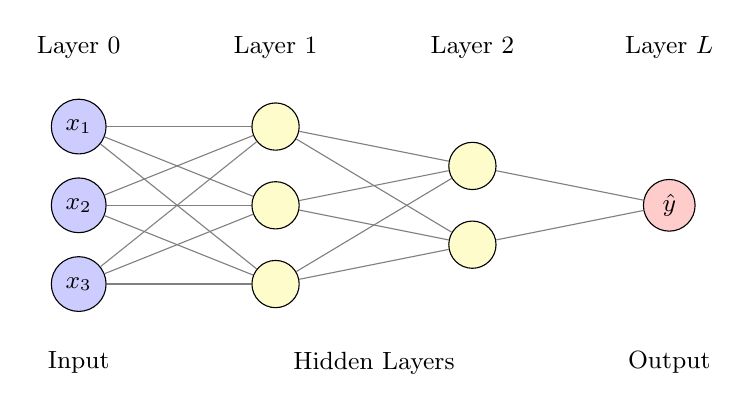
\begin{tikzpicture}[
    input/.style={circle, draw, fill=blue!20, minimum size=0.6cm, font=\small},
    hidden/.style={circle, draw, fill=yellow!20, minimum size=0.6cm, font=\small},
    output/.style={circle, draw, fill=red!20, minimum size=0.6cm, font=\small}
]
    % Layer labels
    \node at (0, 2.5) {\small Layer 0};
    \node at (2.5, 2.5) {\small Layer 1};
    \node at (5, 2.5) {\small Layer 2};
    \node at (7.5, 2.5) {\small Layer $L$};
    
    % Input layer
    \node[input] (x1) at (0, 1.5) {$x_1$};
    \node[input] (x2) at (0, 0.5) {$x_2$};
    \node[input] (x3) at (0, -0.5) {$x_3$};
    
    % Hidden layer 1
    \node[hidden] (h11) at (2.5, 1.5) {};
    \node[hidden] (h12) at (2.5, 0.5) {};
    \node[hidden] (h13) at (2.5, -0.5) {};
    
    % Hidden layer 2
    \node[hidden] (h21) at (5, 1) {};
    \node[hidden] (h22) at (5, 0) {};
    
    % Output
    \node[output] (y) at (7.5, 0.5) {$\hat{y}$};
    
    % Connections (simplified)
    \foreach \i in {x1, x2, x3} {
        \foreach \j in {h11, h12, h13} {
            \draw[gray, thin] (\i) -- (\j);
        }
    }
    \foreach \i in {h11, h12, h13} {
        \foreach \j in {h21, h22} {
            \draw[gray, thin] (\i) -- (\j);
        }
    }
    \foreach \i in {h21, h22} {
        \draw[gray, thin] (\i) -- (y);
    }
    
    % Labels below
    \node at (0, -1.5) {\small Input};
    \node at (3.75, -1.5) {\small Hidden Layers};
    \node at (7.5, -1.5) {\small Output};
\end{tikzpicture}
\end{center}

\subsection{Weight Matrix Notation}

\begin{definitionbox}[Weight Matrix $\mat{W}^{[l]}$]
The weight matrix $\mat{W}^{[l]}$ contains weights connecting layer $l-1$ to layer $l$:
\[
\mat{W}^{[l]} \in \R^{n^{[l]} \times n^{[l-1]}}
\]

Element $W_{ij}^{[l]}$ is the weight from neuron $j$ in layer $l-1$ to neuron $i$ in layer $l$.
\end{definitionbox}

\textbf{Indexing convention}: The destination neuron index comes first (row), then the source neuron index (column). This facilitates matrix multiplication in the forward pass.

\subsection{Bias Vector Notation}

\begin{definitionbox}[Bias Vector $\vect{b}^{[l]}$]
The bias vector for layer $l$:
\[
\vect{b}^{[l]} \in \R^{n^{[l]}}
\]

Element $b_i^{[l]}$ is the bias for neuron $i$ in layer $l$.
\end{definitionbox}

\subsection{Activation Notation}

\begin{definitionbox}[Pre-activation and Activation]
For layer $l$:
\begin{itemize}
    \item \textbf{Pre-activation} (before nonlinearity):
    \[
    \vect{a}^{[l]} = \mat{W}^{[l]} \vect{h}^{[l-1]} + \vect{b}^{[l]}
    \]
    
    \item \textbf{Activation} (after nonlinearity):
    \[
    \vect{h}^{[l]} = \sigma(\vect{a}^{[l]})
    \]
\end{itemize}

Note: $\vect{h}^{[0]} = \vect{x}$ (the input).
\end{definitionbox}

\subsection{Summary of Notation}

\begin{center}
\renewcommand{\arraystretch}{1.3}
\begin{tabular}{|c|c|c|}
\hline
\textbf{Symbol} & \textbf{Meaning} & \textbf{Dimensions} \\ \hline
$L$ & Number of layers (excluding input) & Scalar \\ \hline
$n^{[l]}$ & Number of neurons in layer $l$ & Scalar \\ \hline
$\mat{W}^{[l]}$ & Weight matrix for layer $l$ & $n^{[l]} \times n^{[l-1]}$ \\ \hline
$\vect{b}^{[l]}$ & Bias vector for layer $l$ & $n^{[l]} \times 1$ \\ \hline
$\vect{a}^{[l]}$ & Pre-activation (linear output) & $n^{[l]} \times 1$ \\ \hline
$\vect{h}^{[l]}$ & Activation (hidden output) & $n^{[l]} \times 1$ \\ \hline
$\vect{h}^{[0]} = \vect{x}$ & Input & $n^{[0]} \times 1$ \\ \hline
$\vect{h}^{[L]} = \hat{\vect{y}}$ & Network output & $n^{[L]} \times 1$ \\ \hline
\end{tabular}
\end{center}

% ============================================================================
% FORWARD PROPAGATION
% ============================================================================

\section{Forward Propagation in MLPs}

\subsection{The Algorithm}

\begin{tcolorbox}[title=Forward Propagation Algorithm]
\textbf{Input}: $\vect{x}$ (input features), $\{\mat{W}^{[l]}, \vect{b}^{[l]}\}_{l=1}^{L}$ (parameters)

\textbf{Output}: $\hat{\vect{y}}$ (prediction)

\begin{enumerate}
    \item Set $\vect{h}^{[0]} = \vect{x}$
    \item For $l = 1, 2, \ldots, L$:
    \begin{enumerate}
        \item Compute pre-activation: $\vect{a}^{[l]} = \mat{W}^{[l]} \vect{h}^{[l-1]} + \vect{b}^{[l]}$
        \item Apply activation: $\vect{h}^{[l]} = \sigma(\vect{a}^{[l]})$
    \end{enumerate}
    \item Return $\hat{\vect{y}} = \vect{h}^{[L]}$
\end{enumerate}
\end{tcolorbox}

\subsection{Matrix Formulation}

For a batch of $m$ examples, we can process all inputs simultaneously:

\[
\mat{H}^{[0]} = \mat{X} \in \R^{n^{[0]} \times m}
\]

\[
\mat{A}^{[l]} = \mat{W}^{[l]} \mat{H}^{[l-1]} + \vect{b}^{[l]} \mathbf{1}^\top
\]

\[
\mat{H}^{[l]} = \sigma(\mat{A}^{[l]})
\]

This matrix formulation enables efficient computation on GPUs.

\subsection{Python Implementation}

\begin{lstlisting}[language=Python, caption=Forward Propagation]
import numpy as np

def forward_pass(X, weights, biases, activation=sigmoid):
    """
    Compute forward pass through an MLP.
    
    Args:
        X: Input data (n_features, n_samples)
        weights: List of weight matrices [W1, W2, ..., WL]
        biases: List of bias vectors [b1, b2, ..., bL]
        activation: Activation function
    
    Returns:
        List of activations [h0, h1, ..., hL]
    """
    H = [X]  # h0 = X
    
    for l in range(len(weights)):
        # Pre-activation
        A = weights[l] @ H[l] + biases[l]
        
        # Activation
        H.append(activation(A))
    
    return H
\end{lstlisting}

% ============================================================================
% REPRESENTATIONAL POWER
% ============================================================================

\section{Representational Power}

\subsection{Universal Approximation Theorem}

A profound result in neural network theory:

\begin{theorembox}[Universal Approximation Theorem (Informal)]
A feedforward neural network with a single hidden layer containing a finite number of neurons can approximate any continuous function on compact subsets of $\R^n$, under mild assumptions on the activation function.
\end{theorembox}

This means MLPs are \textbf{universal function approximators}---they can theoretically represent any function we might want to learn.

\begin{importantbox}[Existence vs. Learnability]
The Universal Approximation Theorem only guarantees \textit{existence} of a good network. It says nothing about:
\begin{itemize}
    \item How many neurons are needed
    \item Whether we can \textit{find} the right weights through training
    \item Whether the solution will generalize to new data
\end{itemize}

In practice, deeper networks with fewer neurons per layer often work better than shallow, wide networks.
\end{importantbox}

\subsection{Why Depth Helps}

Deep networks have advantages over shallow ones:

\begin{enumerate}
    \item \textbf{Hierarchical features}: Each layer can learn increasingly abstract representations
    \item \textbf{Efficiency}: Some functions require exponentially fewer neurons when represented with depth
    \item \textbf{Modularity}: Lower layers can be reused for different tasks (transfer learning)
\end{enumerate}

% ============================================================================
% THE NEED FOR SMOOTH ACTIVATIONS
% ============================================================================

\section{From Step Functions to Smooth Activations}

\subsection{Problems with the Step Function}

Recall the perceptron's activation function:
\[
g(z) = \begin{cases} 1 & \text{if } z \geq 0 \\ 0 & \text{otherwise} \end{cases}
\]

This step function has significant drawbacks:

\begin{enumerate}
    \item \textbf{Not differentiable}: The step function has an undefined derivative at $z = 0$ and zero derivative everywhere else. This prevents gradient-based learning.
    
    \item \textbf{Non-smooth}: Small changes in weights can cause large jumps in output.
    
    \item \textbf{No gradient signal}: When $z \neq 0$, the derivative is zero, providing no information about how to improve weights.
\end{enumerate}

\begin{bluebox}[Why Differentiability Matters]
Modern neural network training relies on \textbf{gradient descent}---an optimization algorithm that uses derivatives to find optimal weights. If the activation function isn't differentiable, we cannot compute how changes in weights affect the output, making learning impossible.

The derivative tells us: ``If I increase this weight by a tiny amount, how much will the output change?'' This information is essential for learning.
\end{bluebox}

\subsection{Desirable Properties of Activation Functions}

An ideal activation function should be:

\begin{enumerate}
    \item \textbf{Smooth (continuous)}: No jumps or discontinuities
    \item \textbf{Differentiable}: Has a well-defined derivative everywhere (or almost everywhere)
    \item \textbf{Nonlinear}: Without nonlinearity, neural networks collapse to linear models
    \item \textbf{Bounded outputs}: Prevents exploding activations (for some functions)
    \item \textbf{Computationally efficient}: Fast to compute
\end{enumerate}

% ============================================================================
% THE SIGMOID FUNCTION
% ============================================================================

\section{The Sigmoid Function}

\subsection{Definition}

\begin{definitionbox}[Sigmoid Function]
The \textbf{sigmoid function} (also called the logistic function) is defined as:
\[
\sigma(z) = \frac{1}{1 + e^{-z}}
\]
where $z = \vect{w}^\top \vect{x} + b$ (the weighted sum plus bias).
\end{definitionbox}

\subsection{Properties of Sigmoid}

\begin{center}
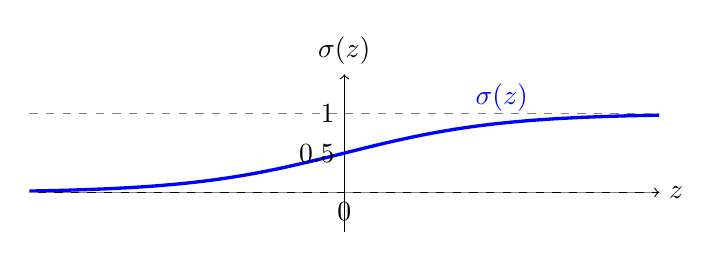
\begin{tikzpicture}
    \draw[->] (-4,0) -- (4,0) node[right] {$z$};
    \draw[->] (0,-0.5) -- (0,1.5) node[above] {$\sigma(z)$};
    
    % Sigmoid curve
    \draw[very thick, blue, domain=-4:4, samples=100] plot (\x, {1/(1+exp(-\x))});
    
    % Asymptotes
    \draw[dashed, gray] (-4,1) -- (4,1);
    \draw[dashed, gray] (-4,0) -- (4,0);
    
    % Labels
    \node[left] at (0,1) {$1$};
    \node[left] at (0,0.5) {$0.5$};
    \node[below] at (0,0) {$0$};
    
    % Annotation
    \node[blue, above] at (2,0.9) {$\sigma(z)$};
\end{tikzpicture}
\end{center}

\textbf{Key Properties:}

\begin{enumerate}
    \item \textbf{Range}: $\sigma(z) \in (0, 1)$ for all $z \in \R$
    \item \textbf{Sigmoid(0) = 0.5}: The function is centered at zero
    \item \textbf{Monotonically increasing}: Larger inputs yield larger outputs
    \item \textbf{S-shaped curve}: Smooth transition from 0 to 1
    \item \textbf{Asymptotes}: $\lim_{z \to -\infty} \sigma(z) = 0$ and $\lim_{z \to \infty} \sigma(z) = 1$
\end{enumerate}

\subsection{Derivative of Sigmoid}

A remarkable property of the sigmoid function is that its derivative has a simple form:

\begin{theorembox}[Sigmoid Derivative]
\[
\sigma'(z) = \sigma(z) \cdot (1 - \sigma(z))
\]
\end{theorembox}

\begin{proof}
Let $\sigma(z) = \frac{1}{1 + e^{-z}} = (1 + e^{-z})^{-1}$.

Using the chain rule:
\begin{align*}
\sigma'(z) &= -(1 + e^{-z})^{-2} \cdot (-e^{-z}) \\
&= \frac{e^{-z}}{(1 + e^{-z})^2} \\
&= \frac{1}{1 + e^{-z}} \cdot \frac{e^{-z}}{1 + e^{-z}} \\
&= \sigma(z) \cdot \frac{e^{-z}}{1 + e^{-z}} \\
&= \sigma(z) \cdot \frac{1 + e^{-z} - 1}{1 + e^{-z}} \\
&= \sigma(z) \cdot \left(1 - \frac{1}{1 + e^{-z}}\right) \\
&= \sigma(z) \cdot (1 - \sigma(z))
\end{align*}
\end{proof}

This elegant form makes gradient computation efficient: once we compute $\sigma(z)$, the derivative is trivial to obtain.

\subsection{Python Implementation}

\begin{lstlisting}[language=Python, caption=Sigmoid Function Implementation]
import numpy as np

def sigmoid(z):
    """Compute the sigmoid of z."""
    return 1 / (1 + np.exp(-z))

def sigmoid_derivative(z):
    """Compute the derivative of sigmoid."""
    s = sigmoid(z)
    return s * (1 - s)
\end{lstlisting}

% ============================================================================
% THE SIGMOID NEURON
% ============================================================================

\section{The Sigmoid Neuron}

\subsection{Architecture}

A \textbf{sigmoid neuron} replaces the step activation with the sigmoid function:

\[
y = \sigma(\vect{w}^\top \vect{x} + b) = \frac{1}{1 + e^{-(\vect{w}^\top \vect{x} + b)}}
\]

\begin{center}
\begin{tikzpicture}[
    input/.style={circle, draw, fill=blue!20, minimum size=0.8cm},
    neuron/.style={circle, draw, fill=yellow!30, minimum size=1.2cm}
]
    \node[input] (x1) at (-2, 1) {$x_1$};
    \node[input] (x2) at (-2, 0) {$x_2$};
    \node[input] (xn) at (-2, -1) {$x_n$};
    \node at (-2, 0.5) {$\vdots$};
    
    \node[neuron] (n) at (1, 0) {$\sigma$};
    
    \node at (3, 0) {$y = \sigma(z)$};
    
    \draw[-Stealth] (x1) -- node[above, sloped] {\small$w_1$} (n);
    \draw[-Stealth] (x2) -- node[above, sloped] {\small$w_2$} (n);
    \draw[-Stealth] (xn) -- node[above, sloped] {\small$w_n$} (n);
    \draw[-Stealth] (n) -- (2.5, 0);
    
    \node[below] at (1, -1) {\small$z = \sum w_i x_i + b$};
\end{tikzpicture}
\end{center}

\subsection{Interpreting Sigmoid Output}

The sigmoid output has a natural interpretation:

\begin{itemize}
    \item Output $\approx 0$: Strong confidence in class 0
    \item Output $\approx 0.5$: Uncertain (at the decision boundary)
    \item Output $\approx 1$: Strong confidence in class 1
\end{itemize}

This makes sigmoid ideal for \textbf{binary classification} problems.

% ============================================================================
% LOSS FUNCTIONS
% ============================================================================

\section{Loss Functions}

\subsection{Why Loss Functions?}

A loss function measures how ``wrong'' our predictions are. It quantifies the discrepancy between:
\begin{itemize}
    \item $\hat{y}$ (predicted output)
    \item $y$ (true label)
\end{itemize}

The goal of learning is to \textit{minimize} the loss.

\subsection{Mean Squared Error (MSE)}

\begin{definitionbox}[Mean Squared Error]
For a dataset with $N$ examples:
\[
\mathcal{L}_{MSE} = \frac{1}{N} \sum_{i=1}^{N} (\hat{y}_i - y_i)^2
\]
where $\hat{y}_i = \sigma(\vect{w}^\top \vect{x}_i + b)$ is the predicted value.
\end{definitionbox}

\subsection{Properties of MSE}

\begin{itemize}
    \item \textbf{Non-negative}: Always $\geq 0$
    \item \textbf{Zero at perfect prediction}: $\mathcal{L} = 0$ when $\hat{y}_i = y_i$ for all $i$
    \item \textbf{Penalizes large errors more}: Squaring amplifies large discrepancies
    \item \textbf{Differentiable}: Enables gradient-based optimization
\end{itemize}

\begin{lstlisting}[language=Python, caption=Mean Squared Error Implementation]
def mse_loss(y_pred, y_true):
    """Compute Mean Squared Error loss."""
    return np.mean((y_pred - y_true) ** 2)
\end{lstlisting}

% ============================================================================
% THE FORWARD PASS
% ============================================================================

\section{The Forward Pass}

\subsection{Definition}

The \textbf{forward pass} is the process of computing the output of a neural network given an input. Information flows from input to output through:

\begin{enumerate}
    \item \textbf{Aggregation}: Compute $z = \vect{w}^\top \vect{x} + b$
    \item \textbf{Activation}: Apply $\hat{y} = \sigma(z)$
    \item \textbf{Loss computation}: Calculate $\mathcal{L}(\hat{y}, y)$
\end{enumerate}

\begin{center}
\begin{tikzpicture}[
    box/.style={draw, rounded corners, minimum width=2cm, minimum height=1cm, align=center, fill=gray!10},
    arrow/.style={-Stealth, thick}
]
    \node[box, fill=blue!20] (input) at (0,0) {Input\\$\vect{x}$};
    \node[box, fill=yellow!20] (agg) at (3,0) {Aggregation\\$z = \vect{w}^\top\vect{x} + b$};
    \node[box, fill=green!20] (act) at (6.5,0) {Activation\\$\hat{y} = \sigma(z)$};
    \node[box, fill=red!20] (loss) at (10,0) {Loss\\$\mathcal{L}$};
    
    \draw[arrow] (input) -- (agg);
    \draw[arrow] (agg) -- (act);
    \draw[arrow] (act) -- (loss);
\end{tikzpicture}
\end{center}

\subsection{Example: Forward Pass by Hand}

Consider three data points:
\begin{itemize}
    \item $(x_1, y_1) = (0.5, 1)$
    \item $(x_2, y_2) = (2.0, 0)$
    \item $(x_3, y_3) = (-1.0, 1)$
\end{itemize}

With initial weights $w = -3.21$ and bias $b = 1.83$:

\textbf{For point 1}:
\begin{align*}
z_1 &= w \cdot x_1 + b = -3.21 \times 0.5 + 1.83 = 0.225 \\
\hat{y}_1 &= \sigma(0.225) = \frac{1}{1 + e^{-0.225}} \approx 0.556 \\
\mathcal{L}_1 &= (\hat{y}_1 - y_1)^2 = (0.556 - 1)^2 \approx 0.197
\end{align*}

Repeat for all points and compute MSE:
\[
\text{MSE} = \frac{0.197 + 0.0001 + 0.004}{3} \approx 0.067
\]

% ============================================================================
% OTHER ACTIVATION FUNCTIONS
% ============================================================================

\section{Other Activation Functions}

While sigmoid is historically important, modern networks use various activation functions:

\subsection{Tanh (Hyperbolic Tangent)}

\[
\tanh(z) = \frac{e^z - e^{-z}}{e^z + e^{-z}} = 2\sigma(2z) - 1
\]

\textbf{Range}: $(-1, 1)$. Zero-centered, which can help learning.

\subsection{ReLU (Rectified Linear Unit)}

\[
\relu(z) = \max(0, z)
\]

\textbf{Range}: $[0, \infty)$. Simple, fast, and works well in practice. Currently the default choice for hidden layers.

\subsection{Comparison}

\begin{center}
\begin{tabular}{|c|c|c|c|}
\hline
\textbf{Function} & \textbf{Range} & \textbf{Pros} & \textbf{Cons} \\ \hline
Sigmoid & $(0,1)$ & Probabilistic output & Vanishing gradient \\ \hline
Tanh & $(-1,1)$ & Zero-centered & Vanishing gradient \\ \hline
ReLU & $[0,\infty)$ & Fast, no saturation & Dead neurons \\ \hline
\end{tabular}
\end{center}

% ============================================================================
% SUMMARY
% ============================================================================

\section{Chapter Summary}

\begin{itemize}
    \item \textbf{Multiple layers} enable solving non-linearly separable problems like XOR.
    
    \item Neural networks are \textbf{directed acyclic graphs (DAGs)} with source (input) and sink (output) nodes.
    
    \item \textbf{Depth} = number of edges on longest path from input to output. Deep networks have depth $> 2$.
    
    \item \textbf{Standard notation}:
    \begin{itemize}
        \item $\mat{W}^{[l]}$: Weight matrix for layer $l$
        \item $\vect{b}^{[l]}$: Bias vector for layer $l$
        \item $\vect{a}^{[l]}$: Pre-activation, $\vect{h}^{[l]}$: Activation
    \end{itemize}
    
    \item \textbf{Forward propagation}: Sequential computation through layers:
    \[
    \vect{a}^{[l]} = \mat{W}^{[l]} \vect{h}^{[l-1]} + \vect{b}^{[l]}, \quad \vect{h}^{[l]} = \sigma(\vect{a}^{[l]})
    \]
    
    \item \textbf{Universal Approximation}: MLPs can approximate any continuous function, but finding good weights remains the challenge.
    
    \item \textbf{Step functions} are problematic because they have zero gradients almost everywhere, making gradient-based learning impossible.
    
    \item \textbf{Sigmoid} $\sigma(z) = \frac{1}{1+e^{-z}}$ is smooth, differentiable, and maps any real number to $(0,1)$.
    
    \item \textbf{Sigmoid's derivative} has the elegant form: $\sigma'(z) = \sigma(z)(1-\sigma(z))$.
    
    \item \textbf{Loss functions} (like MSE) quantify prediction error and provide the objective to minimize during training.
    
    \item The \textbf{forward pass} computes predictions: input $\rightarrow$ aggregation $\rightarrow$ activation $\rightarrow$ output.
    
    \item Other activations (Tanh, ReLU) address sigmoid limitations and are commonly used in modern networks.
\end{itemize}

\begin{bluebox}[Looking Ahead]
We now understand how information flows forward through a network. The next critical question is: \textbf{How do we learn the weights?}

This leads us to:
\begin{enumerate}
    \item \textbf{Gradient Descent}: The optimization algorithm
    \item \textbf{Backpropagation}: Efficient gradient computation
\end{enumerate}
\end{bluebox}
